\documentclass[a4paper]{article}

\usepackage[utf8]{inputenc}
\usepackage[T1]{fontenc}
\usepackage{textcomp}
\usepackage{amsmath, amssymb, amsthm}
\usepackage[style=alphabetic]{biblatex}
\usepackage{setspace}
\usepackage{tikz}
\addbibresource{sources.bib}
\usetikzlibrary{automata, arrows, chains}
\tikzset{
	>=stealth, % makes the arrow heads bold
	node distance=3cm, % specifies the minimum distance between two nodes. Change if necessary.
	every state/.style={thick, fill=gray!10}, % sets the properties for each ’state’ node
	initial text=$ $, % sets the text that appears on the start arrow
	in place/.style={
		auto=false,
		inner sep=3pt,
	},
}

% figure support
\usepackage{import}
\usepackage{xifthen}
\pdfminorversion=7
\usepackage{pdfpages}
\usepackage{transparent}
\usepackage{float}
\newcommand{\incfig}[1]{%
	\def\svgwidth{\columnwidth}
	\import{./figures/}{#1.pdf_tex}
}

\pdfsuppresswarningpagegroup=1

\title{Project 1}
\date{Oct 26, 2022}
\author{Jack Ruder}


\begin{document}

\doublespacing
\maketitle


\section{Introduction}
In this report we detail how to use multiple linear regression to create a linear model. Our goal will be to model the gas milage of cars, using the mtcars dataset built into R. We will detail the modeling process, interpretation of the model, and analysis of the resulting statistics. 

\section{Background}
The mtcars dataset includes 32 observations, on 11 numeric variables. In a snapshot of the data,
\begin{figure}[H]
\centering
	\begin{tabular}{l|r|r|r|r|r|r|r|r|r|r|r}
	\hline
	  & mpg & cyl & disp & hp & drat & wt & qsec & vs & am & gear & carb\\
	\hline
	Mazda RX4 & 21.0 & 6 & 160.0 & 110 & 3.90 & 2.620 & 16.46 & 0 & 1 & 4 & 4\\
	\hline
	Mazda RX4 Wag & 21.0 & 6 & 160.0 & 110 & 3.90 & 2.875 & 17.02 & 0 & 1 & 4 & 4\\
	\hline
	Datsun 710 & 22.8 & 4 & 108.0 & 93 & 3.85 & 2.320 & 18.61 & 1 & 1 & 4 & 1\\
	\hline
	Hornet 4 Drive & 21.4 & 6 & 258.0 & 110 & 3.08 & 3.215 & 19.44 & 1 & 0 & 3 & 1\\
	\hline
	Hornet Sportabout & 18.7 & 8 & 360.0 & 175 & 3.15 & 3.440 & 17.02 & 0 & 0 & 3 & 2\\
	\hline
	\end{tabular}
	\caption{Snapshot of mtcars Dataset}
	\label{fig:mtcars-snap}
\end{figure}
we see our Response Variable represented by mpg, and 10 other possible explanatory variables. These are:
\begin{itemize}
	\item mpg: Miles/(US) gallon
	\item cyl:   Number of cylinders                      
	\item disp:  Displacement (cu.in.)                    
	\item hp:    Gross horsepower                         
	\item drat:  Rear axle ratio                          
	\item wt:    Weight (1000 lbs)                        
	\item qsec:  1/4 mile time                            
	\item vs:    Engine (0 = V-shaped, 1 = straight)      
	\item am:    Transmission (0 = automatic, 1 = manual) 
	\item gear:  Number of forward gears                  
	\item carb:  Number of carburetors                    
\end{itemize}
This data, found in the 1974 Motor Trend magazine, shows cars from 1973-74 \cite{data}. 

\section{Analysis}
We begin by exploring the distribution of variables in the data, as well as observing relationships between them.
Observe in figure 2 that density plots of each variable are placed along the diagonal, and relationships between pairs of variables are expressed by scatter plots and \(R^2\) values.
\begin{figure}[H]
	\centering
	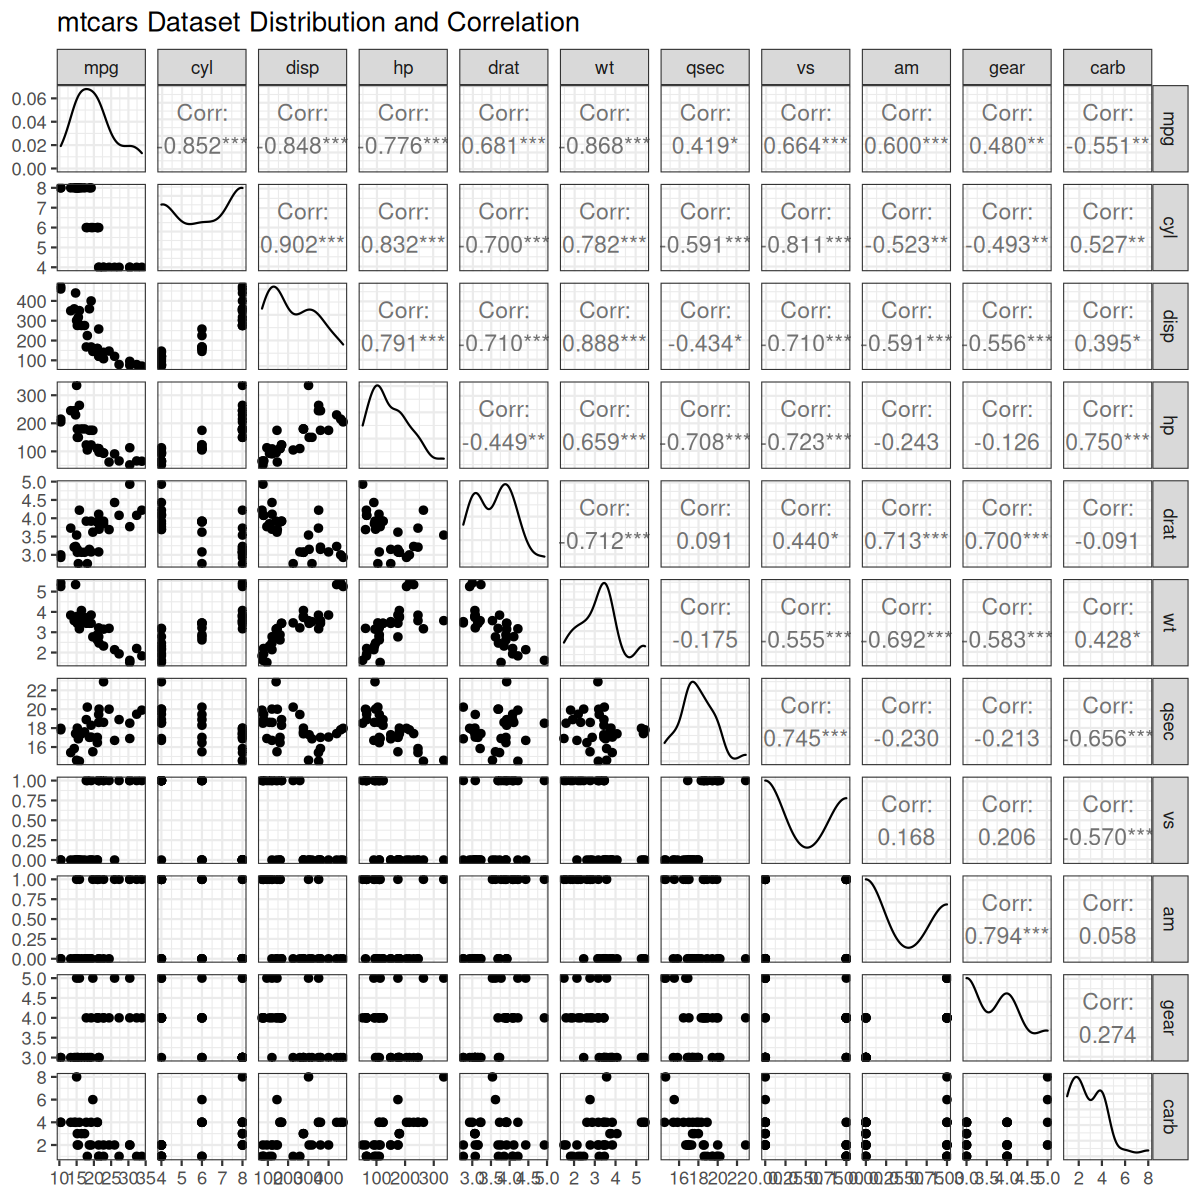
\includegraphics[width=0.9\textwidth]{"../corrplot.png"}
	\caption{Correlation and Density Plots}
	\label{fig:Correlation-and-Density-Plots}
\end{figure}
Many of the distributions show right skews. These are mpg, disp, hp, drat, wt, qsec and carb, although wt and qsec are potentially normally distributed with exception of a few outliers. Log transforming these variables shows an improvement in normality, 
\begin{figure}[H]
	\centering
	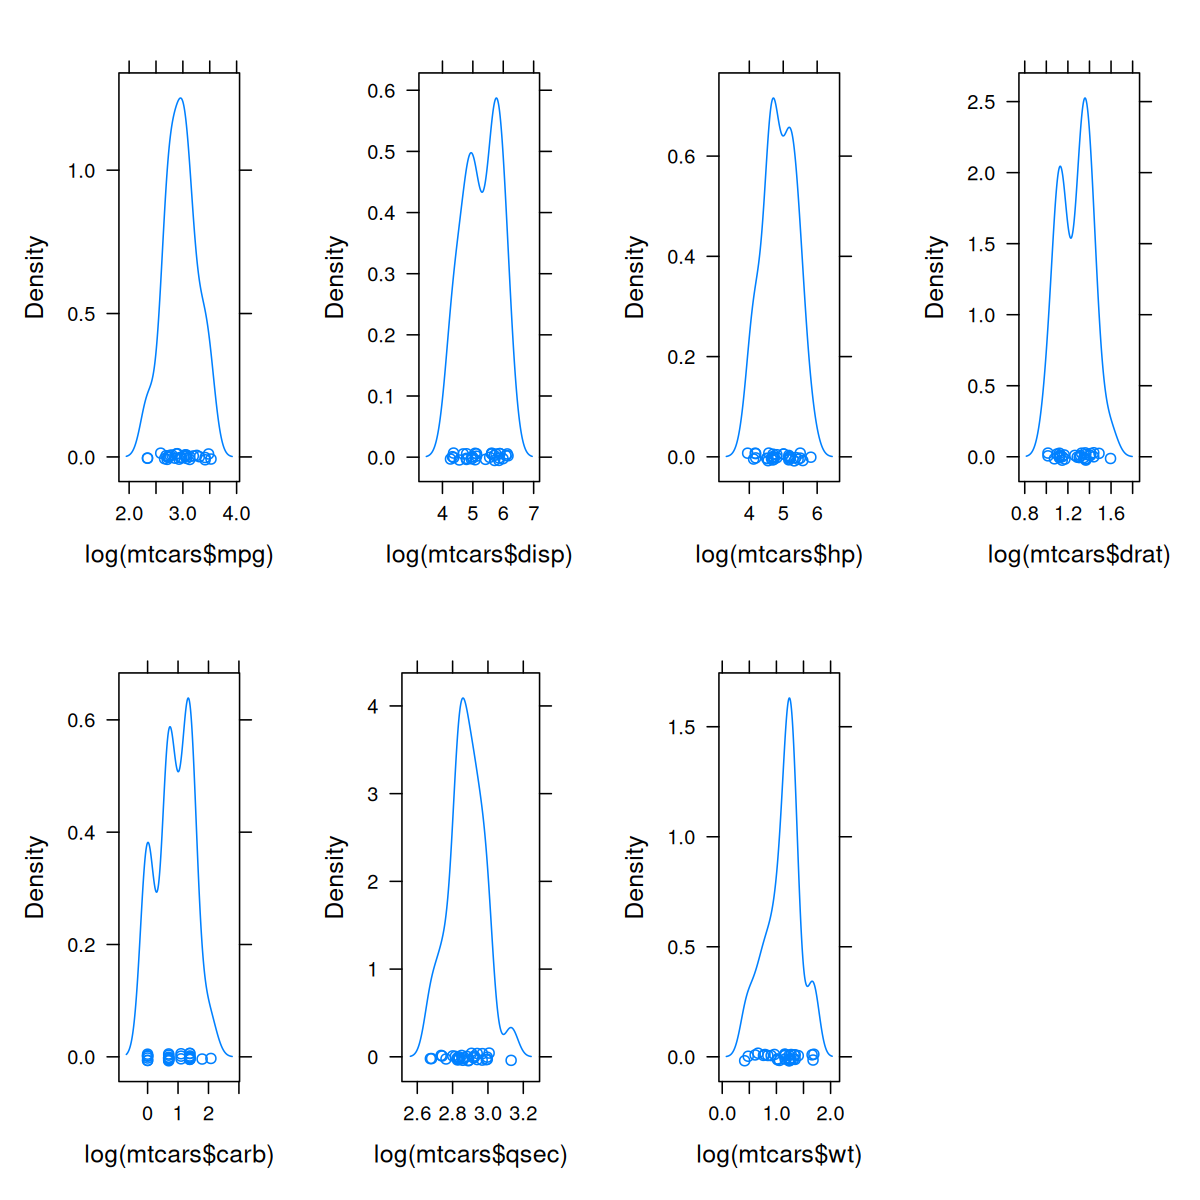
\includegraphics[width=0.8\textwidth]{"../transformedDensities.png"}
	\caption{Log-Transformed Variables}
	\label{fig:Log-Transformed-Variables}
\end{figure}

other than for qsec where the distribution does not change much.

Again, there are only 32 observations. To avoid overfitting a model, we should limit ourselves to no more than 4 predictors, ideally fewer. A useful observation is that qsec, gear, carb are not very correlated with mpg, showing correlations of \(<0.6\). Thus we should be safe in leaving them out of our model. 

We begin by constructing a model with the most relevant-appearing terms. We have
\begin{equation}
\log mpg = \beta_0 + \beta_1 \log wt + \beta_2 cyl +\beta_3\log(hp) \beta_4 \log disp + \beta_5 \log drat + \beta_6 vs + \beta_7 am.
\end{equation}
We use R \cite{r} to fit this model, providing an Adjusted R-squared of 0.852. Then we check the variance inflation factor of each variable, using the car package. There were two variables with a VIF over 10, \(cyl\) at 12.45 and \(\log disp\) at 18.69. This suggests that \(cyl\) and \(\log disp\) are very correlated with the rest of the data. We will begin by removing \(\log disp\), and refitting the model. 

The resulting model showed a drop in the multiple R-squared from 0.8855 to 0.8845, meaning removing \(\log disp\) was a relatively insignificant change, as expected. 

Checking the VIF again shows \(cyl\) as the only variable with a VIF over 10. We will remove it.
This time, the drop in the multiple R-squared was to 0.8842, an even smaller change. The VIF 
with \(\log disp\) and \(cyl\) removed shows all predictors under a score of \(4.9\), meaning collinearity is largely gone from our model. The form of model at this stage is 
\begin{equation}
\log mpg = \beta_0 + \beta_1 \log wt + \beta_2\log hp + \beta_3 \log drat + \beta_4 vs + \beta_5 am.
\end{equation}
Lastly, we observe in the variance table for the fitted model that \(\log drat\), \(vs\), and \(am\) show F values of less than 1, meaning they account for less error than the residuals themselves. We should definitely remove these. 

This gives the following model, 
\begin{equation}
	\log mpg = \beta_0 + \beta_1 \log wt + \beta_2 \log hp.
\end{equation}
Performing a nested F-test between this model and the immediate previous model gives a \(p\)-value of 0.9608, meaning we accept the null hypothesis that the more complex model is not substantially better than the model with \(\log drat\), \(vs\), and \(am\) removed. Compared to the model with all terms, we have a \(p\)-value of \(0.98\), strong evidence that leaving out the other terms is useful.

The fit for our model, using multiple linear regression, is
\begin{equation}
	\log mpg = 4.83 - 0.56 \log wt -0.26\log hp.
\end{equation}
This model is extremely signifiant with a \(p\)-value of \(3.14\cdot 10^{-14}\), and an F statistic of 109.3 on 2 degrees of freedom. Thus, we reject the null hypothesis that our model explains \(\log mpg\) in its given form. The adjusted R-squared is 0.8748 (compared to 0.852 in the full model), indicating that this model is unlikely to be an overfit. Still, we need to check for normally distributed residuals.
\begin{figure}[H]
	\centering
	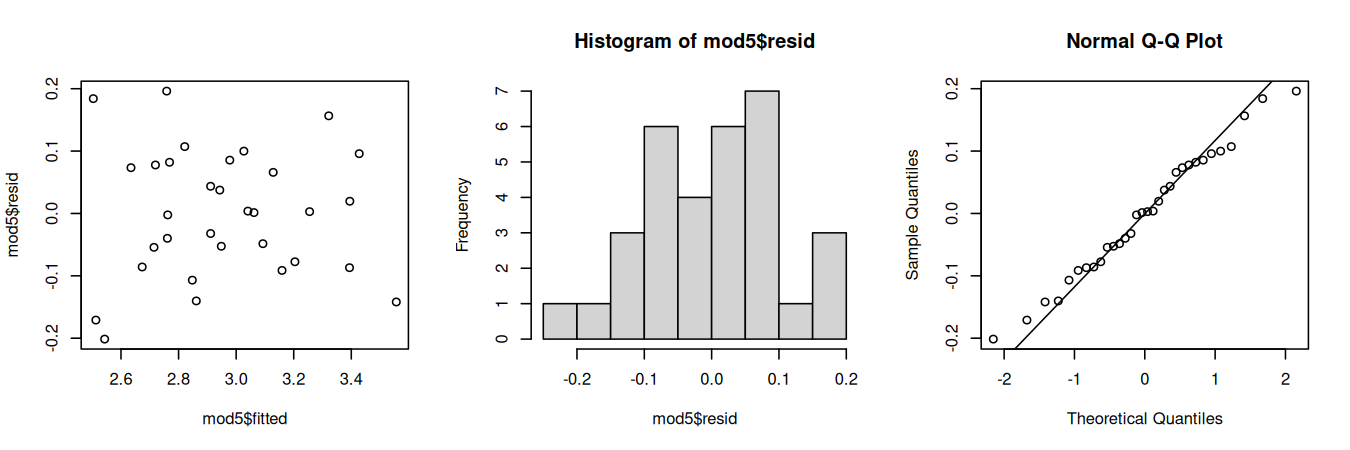
\includegraphics[width=0.9\textwidth]{"../diag.png"}
	\caption{Diagnostic Plots for Residuals}
	\label{fig:diagnose}
\end{figure}
We see, that there appears to be a linear relationship, and the residuals are normally distributed, with exception of a few outliers. 
Constructing a 95\% confidence interval on each of the coefficients in our model gives us
\begin{figure}[H]
\centering
\begin{tabular}{l|c|c}
	-  & 25 & 97.5 \\
	\hline
	\(\beta_0\) & 4.37 & 5.29 \\
	\hline
	\(\beta_1\) & -0.74 & -0.38 \\
	\hline
	\(\beta_2\) & -0.37 & -0.14
\end{tabular}.
\end{figure}

Now, it may be appropriate to reframe our model in terms of \(mpg\). Exponentiating both sides of our model gives
\begin{equation}
	mpg = \frac{125.21}{wt^{0.56}h^{0.26}} \approx \frac{125.21}{\sqrt{wt}\sqrt[4]{hp} }.
\end{equation}
Per our model, since Weight and Horsepower are greater than 1, we should never expect to exceed 125 mpg, though Weight=1000lb and 1 horsepower is an unrealistic scenario for a vehicle. More useful is the idea that our mpg is roughly proportional to \(\frac{1}{\sqrt{wt} }\), and\(\frac{1}{\sqrt[4]{hp} }\). So, when weight quadruples, gas milage halves. Horsepower has less of an effect, you would need 16 times the horsepower to halve the gas milage, according to the model.

It might be nice to get some predictions from our model. We will break the dataset into Compact (<2500 lbs), Midsize (2500-4000 lbs) and Large cars (4000 lbs). The mean 95\% predicted intervals and confidence interval are given in the below table.


\begin{figure}[H]
\centering
\begin{tabular}{c|c|c|c|c|c}
	&fit & \(C_{lwr}\) & \(C_{upr}\) & \(P_{lwr}\) & \(P_{upr}\) \\
	\hline
	Compact &28.19 & 26.21 &30.32 &22.43 & 35.43\\	\hline
	Midsize & 17.86 & 16.87 &18.90 &14.27 & 22.33\\	\hline
	Large & 13.06 & 12.16 &14.04 &10.41 & 16.40
\end{tabular}.
\end{figure}
We see that mpg predictions are well within the expected ranges, and as expected larger cars show a decrease in gas milage. For example, 95\% of new large car observations will have gas milages between 10.41 and 16.40 mpg, versus 22.43 and 35.43 mpg for new compact car observations.

The model has a tighter grip on predicted values for larger cars, 95\% of intervals at the 95\% level will have the mpg fall between \(12.16\) and \(14.04\), quite a tight bound. Likely this is a limitation of the dataset due to the lack of large vehicles, ideally we would expect a wider interval.
\section{Conclusions}
We have shown that the MPG of cars is roughly predicted by 
\begin{equation}
	mpg = \frac{125.21}{\sqrt{wt}\sqrt[4]{hp}}.
\end{equation}
However, arriving at this model meant ignoring many variables to obtain a model that will perfrom well on new data. The size of this dataset was small with only 32 samples, making it difficult to create a more decisive model. However, for other vechicles from 1973-1974, this model should apply, since many cars within the same year are limited by the same kinds of technology. It is hard to discern whether or not these vehicles in the dataset were randomly selected, the best guess is that they were selected to encapsulate all types of vehicles at that time. Thus we could use this model for inference about other vehicles at that time, but extrapolating to modern cars would be a poor choice. We cannot establish any causation, since this is purely an observational study. 

Additionally, it is worth noting that we introduced bias by using backwards selection (eliminating variables) in selecting a multiple linear regression model. It very well could be that weight and horsepower encapsulate the differences in mpg within this dataset, but displacement and axle ratio are more important in another dataset. Again, more datapoints would be useful.

\nocite{*}
\printbibliography

\end{document}
